\documentclass{article}

%math stuff
\usepackage{amsmath}
\usepackage{enumitem}
\usepackage{mathtools}
\usepackage{listings}

%bibliography/appendix
\usepackage{cite}
\usepackage[toc,page]{appendix}

%figures
\usepackage{graphicx}
\usepackage{booktabs}

%General Formating
\renewcommand*\familydefault{\sfdefault}
\usepackage{cmbright}
\usepackage[letterpaper, portrait, margin=1.5in]{geometry}
\usepackage{fancyhdr}
\pagestyle{fancy}

%Header
\lhead{Schulman}
\rhead{Page \thepage}

\title{Econometrics I Homework 1}
\author{Eric Schulman}
\date{\today}

\begin{document}

\maketitle

\section{Part I}

\begin{enumerate}
	\item[2.2] 

	$$E( E(xy | x))$$
	$$ = E( xE(y | x))$$
	$$ = E(a(x+bE(x))|x)$$
	$$= a(x+bE(x))$$
	
	\item[2.4]

	$$E(y|x=0) = E(y^2 |x=0)  = .8$$
	$$E(y|x=1) = E(y^2 |x=1)  = .6$$
	$$E(y^2|x=0) - (E(y|x=0))^2 = .16$$
	$$E(y^2|x=1) - (E(y|x=1))^2 = .24$$

	\item[2.5]
	\begin{enumerate} [label=\alph*)]
    	\item 

    	$$E((e^2-g(x))^2)$$
        
        \item 

        $$\text{Minimize } E((e^2-h(x))^2)$$
        
        \item 

        $$E((e^2-g(x))^2)$$
        $$ = E((e^2-\sigma^2(x) + \sigma^2(x) - h(x))^2)$$
        $$ = E((e^2-\sigma^2(x))^2) + E((\sigma^2(x) -h(x))^2) + 2E((\sigma^2(x) -h(x))(e^2-\sigma^2(x)))$$

        Since $$E((\sigma^2(x) -h(x))(e^2-\sigma^2(x)))$$
        $$ = E(E((\sigma^2(x) -h(x))(e^2-\sigma^2(x))|x))$$
        $$ = E(E(e^2\sigma^2(x) - e^2g(x) + g(x)\sigma^2(x) +\sigma^2(x) \sigma^2(x)|x))$$
        $$ = E(\sigma^2(x)\sigma^2(x) - \sigma^2(x)g(x) + g(x)\sigma^2(x) +\sigma^2(x) \sigma^2(x)) = 0$$

        We have
        $$E((e^2-g(x))^2) = E((e^2-\sigma^2(x))^2) + E((\sigma^2(x) -h(x))^2) \geq E((e^2-\sigma^2(x))^2) $$
    
    \end{enumerate} 

    \item[2.7]

    $$E(y^2|x) - (E(y|x))^2 = \text{Var}(y|x) = \text{Var}(\beta x + e |x) = \text{Var}(e|x) = \sigma^2(x)$$

    \item[2.10] True

    $$E(x^2e) = E(E(e x^2 |x) ) = E( x^2 E(e |x) ) = 0$$

    \item[2.11] False

    Suppose $x$ is distributed $N(0,1)$, $e|x$ is distributed $N(x^2,1)$. Then,

    $$E(xe) = E(E(xe|x) = E(xE(e|x)) = E(x^3) = 0$$

    However,

    $$E(x^2e) = E(E(x^2e|x)) = E(x^2E(e|x)) = E(x^4) = 3\sigma ^{4} = 3 $$ i.e. the fourth moment of the normal distribution

    \item[2.12] False

    Suppose $e|x$ has the distribution $N(0,x^2)$. Then $E(e|x) = 0$, but $x$ and $e$ are not independent.

   
    \item[2.13] False

    Suppose $x$ is distributed $N(0,1)$, $e|x$ is distributed $N(x^2,1)$. Then,

    $$E(ex) = 0$$ (as shown in 2.11)
    $$E(e|x) = x^2$$


    \item[2.14] False

    Consider a distribution where the third conditional moment is a function of x. i.e. 

    $$E(x|e) = 0$$
    $$E(x^2|e) = 0$$
    $$E(x^3|e) = h(x)$$

\end{enumerate}

\section{Part II}
\begin{enumerate}[label=\alph*)]
\item

Below is the histogram. The histogram appears to have 2 peaks.

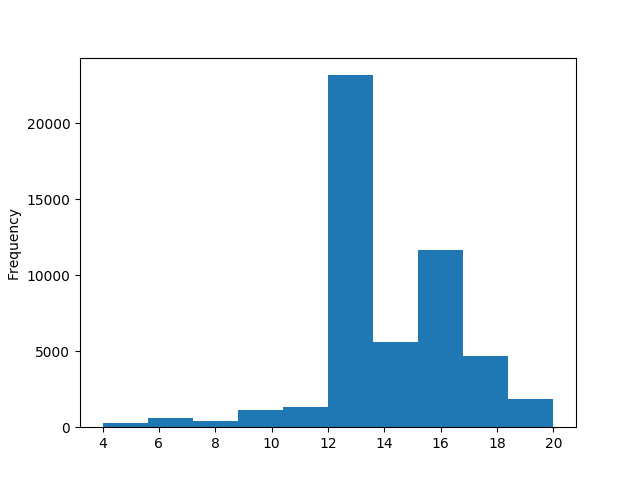
\includegraphics[scale=.8]{part_a}

\item The table below show the results.

\begin{tabular}{ c c }
 Years & Observations \\
 \hline
 12 & 13896 \\ 
 16 & 11640 \\ 
 18 & 4670  \\ 
 20 & 1875 
\end{tabular}


\item

Below are the kernel density plots in order of years of education (i.e. 12, 16, 18, 20).

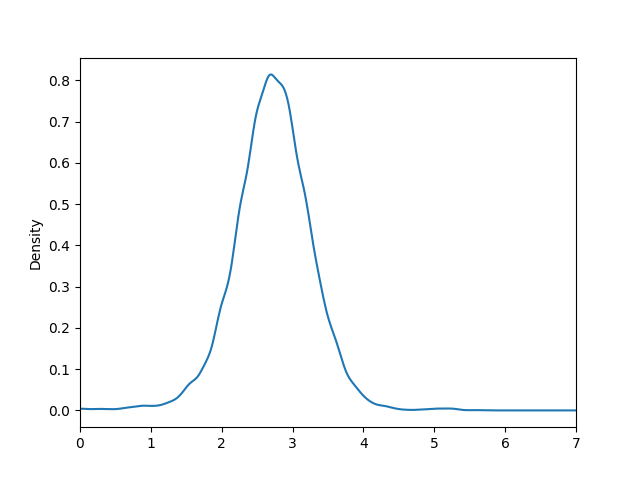
\includegraphics[scale=.8]{part_b_12}

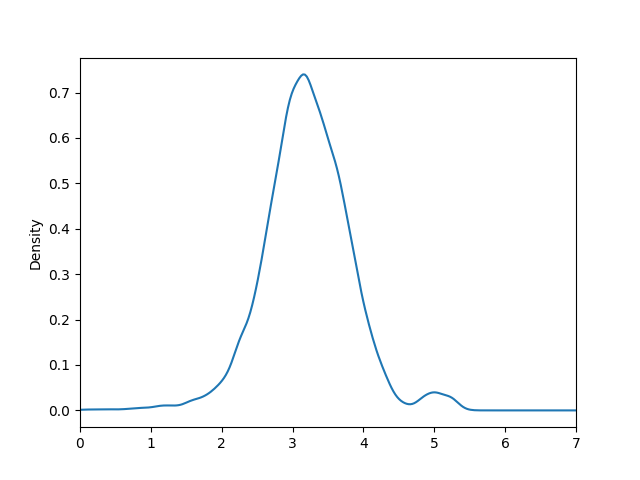
\includegraphics[scale=.8]{part_b_16}

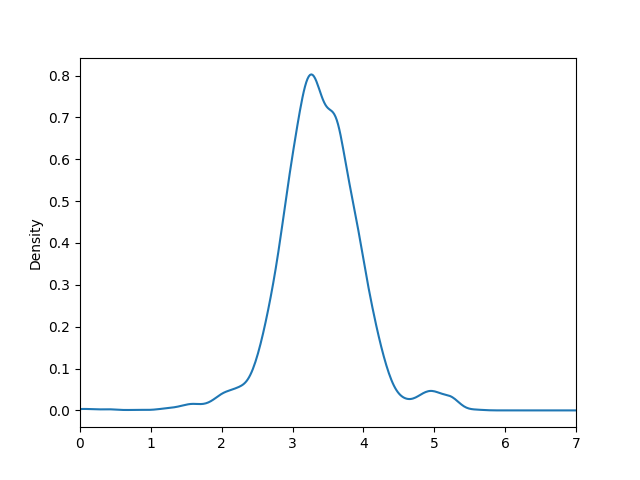
\includegraphics[scale=.8]{part_b_18}

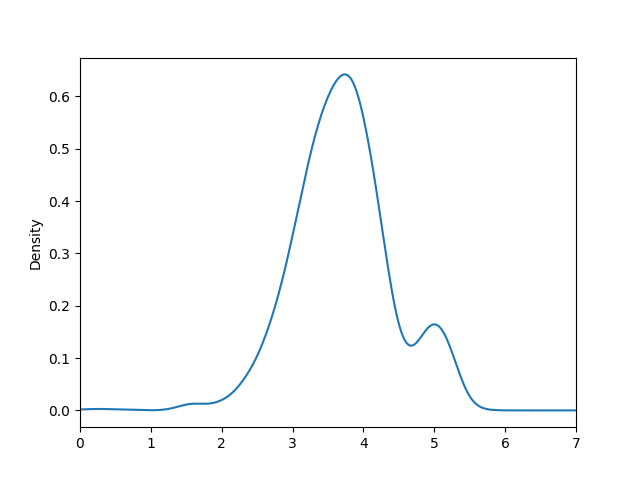
\includegraphics[scale=.8]{part_b_20}

\item The table below show the results.

\begin{tabular}{ c c c }
 Years & Mean & Variance \\
 \hline
 12 & 2.712 & 0.329 \\ 
 16 & 3.201 & 0.416 \\ 
 18 & 3.381 & 0.363 \\ 
 20 & 3.689 & 0.619    
\end{tabular}

By the table, we can see 20 years of education has the highest variance, followed by 16 years of education. 12 years of education has the least variance.


\item The table below show the results.

\begin{tabular}{ c c c c }
Year & 25th & 50th & 75th \\
\hline
12 & 2.403 & 2.733 & 3.055 \\
16 & 2.839 &	3.180 & 3.585 \\
18 & 3.062 &	3.362 & 3.710 \\
20 & 3.275 &	3.690 &	4.089 \\
\end{tabular}

Again the distribution for 20 years of education is has the most dispersion. The highest quartile of 12 years of education make less than the lowest quartile of 20 years of education.

\item The table below show the results.

\begin{tabular}{ c c }
Years & Difference \\
\hline
12 & 0 \\
16 & 0.489 \\
18 & 0.669 \\
20 & 0.977 \\
\end{tabular}

The more education you have the more you are expected to make according to the differences in the table.

\item  The table below show the results.

\begin{tabular}{ c c c c c c } \\ Year 1 & Year 2 & Diff & SE & T-Value & Reject \\ 
 \hline 
12 & 12 & 0.0 & 0.00486691158299 & 0.0 & False \\ 
12 & 16 & -0.488918 & 0.00486691158299 & -100.457462777 & True \\ 
12 & 18 & -0.669176 & 0.00486691158299 & -137.494970241 & True \\ 
12 & 20 & -0.976912 & 0.00486691158299 & -200.725245359 & True \\ 
16 & 12 & 0.488918 & 0.00597543294539 & 81.821282852 & True \\ 
16 & 16 & 0.0 & 0.00597543294539 & 0.0 & False \\ 
16 & 18 & -0.180258 & 0.00597543294539 & -30.1665629463 & True \\ 
16 & 20 & -0.487994 & 0.00597543294539 & -81.6667908266 & True \\ 
18 & 12 & 0.669176 & 0.00882675326792 & 75.8122316274 & True \\ 
18 & 16 & 0.180258 & 0.00882675326792 & 20.4218095382 & True \\ 
18 & 18 & 0.0 & 0.00882675326792 & 0.0 & False \\ 
18 & 20 & -0.307736 & 0.00882675326792 & -34.8640263334 & True \\ 
20 & 12 & 0.976912 & 0.0181678405989 & 53.7714989472 & True \\ 
20 & 16 & 0.487994 & 0.0181678405989 & 26.8603431317 & True \\ 
20 & 18 & 0.307736 & 0.0181678405989 & 16.9385104793 & True \\ 
20 & 20 & 0.0 & 0.0181678405989 & 0.0 & False \\ 
\end{tabular}

\item The table below show the results.

\begin{center}
\begin{tabular}{lclc}
\toprule
\textbf{Dep. Variable:}    &      lwage       & \textbf{  R-squared:         } &     0.203   \\
\textbf{Model:}            &       OLS        & \textbf{  Adj. R-squared:    } &     0.203   \\
\textbf{Method:}           &  Least Squares   & \textbf{  F-statistic:       } &     2727.   \\
\textbf{Date:}             & Sat, 03 Feb 2018 & \textbf{  Prob (F-statistic):} &     0.00    \\
\textbf{Time:}             &     13:45:04     & \textbf{  Log-Likelihood:    } &   -30104.   \\
\textbf{No. Observations:} &       32081      & \textbf{  AIC:               } & 6.022e+04   \\
\textbf{Df Residuals:}     &       32077      & \textbf{  BIC:               } & 6.025e+04   \\
\textbf{Df Model:}         &           3      & \textbf{                     } &             \\
\bottomrule
\end{tabular}
\begin{tabular}{lcccccc}
                  & \textbf{coef} & \textbf{std err} & \textbf{t} & \textbf{P$>$$|$t$|$} & \textbf{[0.025} & \textbf{0.975]}  \\
\midrule
\textbf{const}    &       2.7121  &        0.005     &   516.939  &         0.000        &        2.702    &        2.722     \\
\textbf{educ\_16} &       0.4889  &        0.008     &    62.916  &         0.000        &        0.474    &        0.504     \\
\textbf{educ\_18} &       0.6692  &        0.010     &    63.969  &         0.000        &        0.649    &        0.690     \\
\textbf{educ\_20} &       0.9769  &        0.015     &    64.203  &         0.000        &        0.947    &        1.007     \\
\bottomrule
\end{tabular}
\begin{tabular}{lclc}
\textbf{Omnibus:}       & 10460.946 & \textbf{  Durbin-Watson:     } &     1.767   \\
\textbf{Prob(Omnibus):} &    0.000  & \textbf{  Jarque-Bera (JB):  } & 213631.163  \\
\textbf{Skew:}          &   -1.068  & \textbf{  Prob(JB):          } &      0.00   \\
\textbf{Kurtosis:}      &   15.460  & \textbf{  Cond. No.          } &      4.98   \\
\bottomrule
\end{tabular}
%\caption{OLS Regression Results}
\end{center}



\section{Python Code}

\begin{lstlisting}[language=Python]

import pandas
import matplotlib.pyplot as plt
import statsmodels.api as sm

FNAME = 'cps09mar.dta'
CATEGORIES = [12,16,18,20]

def main():
	#part a
	df = pandas.read_stata(FNAME)
	plt.figure()
	hist = df[(df.educ > 1)]
	hist['educ'].plot.hist()
	plt.savefig('part_a')

	#part b-e
	stats = dict()
	for y in CATEGORIES:
		stats[y] = helper(df,y)

	#write result to file
	result = open("hw1_results.csv","w+")
	result.write('num_obs,mean,var,q25,q50,q75\n')
	for y in CATEGORIES:
		result.write('%s,%s,%s,%s,%s,%s\n'% tuple(stats[y]) )

	result.close()

	#part f-g
	result = open("hw1_results.tex","w+")
	result.write('\\begin{tabular}{ c c c c c c } \\\\')
	result.write(' Year 1 & Year 2 & Diff & SE & T-Value & Reject \\\\ \n \hline \n')
	for y in CATEGORIES:
		for x in CATEGORIES:
			diff = stats[y][1] - stats[x][1]
			se =  (stats[y][2]/stats[y][0])**(.5)
			t_value = diff / se
			reject = (t_value > 2.02) or (t_value < -2.02)
			result.write('%s & %s & %s & %s & %s & %s \\\\ \n'% (y,x,diff,se,t_value,reject) )
	result.write('\\end{tabular}')
	result.close()


def helper(df,y):
	df = df[df.educ == y]
	num_obs = df['educ'].count()

	plt.figure()
	df['lwage'].plot.density()
	plt.xlim(0, 7)
	plt.savefig('part_b_%s'%y)
	
	mean = df['lwage'].mean()
	var = df['lwage'].var()
	
	q25 = df['lwage'].quantile(q=.25)
	q50 = df['lwage'].quantile(q=.5)
	q75 = df['lwage'].quantile(q=.75)

	#last 2 fields to be filled in later
	return [num_obs,mean,var,q25,q50,q75]


def do_regression():
	df = pandas.read_stata(FNAME)
	df = df[(df.educ == 12) | (df.educ == 16)| (df.educ == 18)| (df.educ == 20)]
	
	#set up X matrix
	X = pandas.get_dummies(df['educ'], prefix='educ')
	X = X[['educ_16', 'educ_18', 'educ_20']]
	X = sm.add_constant(X)
	
	y = df['lwage']
	
	#write result
	model_result = sm.OLS(y,X).fit()
	result_doc = open('hw1_reg.tex','w+')
	result_doc.write( model_result.summary().as_latex() )
	result_doc.close()


if __name__ == "__main__":
	main()
	do_regression()

\end{lstlisting}

\end{enumerate}



\end{document}